\chapter{Planificación}
\section[Objectivos]{Objetivos}
Los objetivos concretos que persigue este proyecto son los siguientes:
\begin{enumerate}
	\item Estudio del estado del arte de los sistemas de planificación de rutas con recomendaciones, y de los sistemas de información sobre puntos de interés en las ciudades.
	\item Definición y diseño de modelos y herramientas de recomendación de itinerarios ajustados a las necesidades y preferencias de los turistas.
	\item Validación de modelos y métodos, empleando pruebas y datos de puntos de interés en ciudades de interés turístico.
	\item Obtención de un prototipo software integrado en una aplicación para dispositivos móviles.
	\item Creación de documentación técnica, entregables y memoria final del proyecto.

\section[Diagrama de Gantt]{Diagrama de Gantt}
En esta sección se muestra una diagrama de Gantt con la planificación del proyecto dividido en diferentes tareas.\newline
\begin{figure}[H]
	\centering
	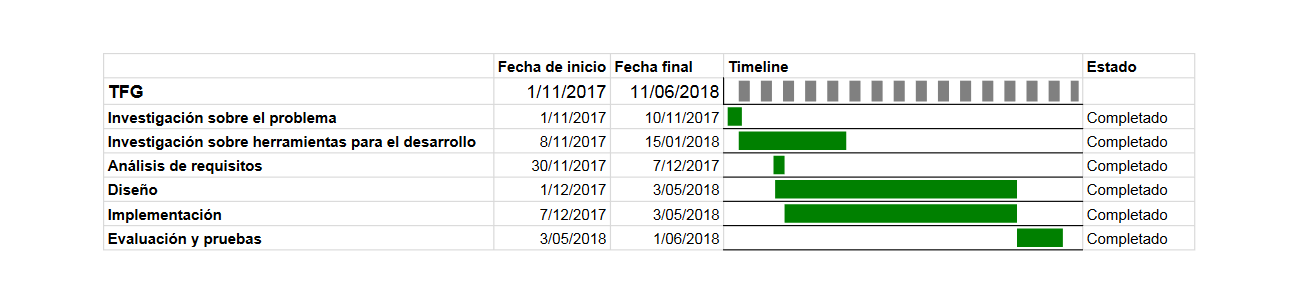
\includegraphics[scale=0.4]{imagenes/Gantt.png}
	\caption{Planificación del proyecto}
	\label{fig:gantt}
\end{figure}
	
\end{enumerate}
